% DeepQuark: Deep-Neural-Network Approach to Multiquark Bound States
% Beamer Presentation for Hadron Physics Workshop
% Based on arXiv:2506.20555

\documentclass[aspectratio=169,10pt]{beamer}

% Theme and colors
\usetheme{Madrid}
\usecolortheme{default}
\definecolor{heavyblue}{RGB}{0,70,140}
\definecolor{lightquarkorange}{RGB}{230,120,50}
\setbeamercolor{structure}{fg=heavyblue}
\setbeamercolor{frametitle}{bg=heavyblue,fg=white}
\setbeamercolor{title}{fg=white,bg=heavyblue}

% Packages
\usepackage{amsmath,amssymb,bm}
\usepackage{graphicx}
\usepackage{tikz}
\usetikzlibrary{arrows.meta,positioning,shapes,calc,decorations.pathmorphing}
\usepackage{multirow}
\usepackage{booktabs}
\usepackage{xcolor}
\usepackage{hyperref}

% Custom commands
\newcommand{\threebar}{\bar{3}_c}
\newcommand{\sixbar}{\bar{6}_c}

% Remove navigation symbols
\setbeamertemplate{navigation symbols}{}

% Add slide numbers
\setbeamertemplate{footline}[frame number]

% Title information
\title[DeepQuark]{DeepQuark: Deep-Neural-Network Approach to\\ Multiquark Bound States}
\author[L.\ Meng]{Wei-Lin Wu$^{1}$, \underline{Lu Meng}$^{2,3}$, Shi-Lin Zhu$^{1,4}$}
\institute[PKU \& RUB]{
$^1$School of Physics, Peking University\\
$^2$Institut f\"ur Theoretische Physik II, Ruhr-Universit\"at Bochum\\
$^3$School of Physics, Southeast University\\
$^4$Center of High Energy Physics, Peking University
}
\date{Hadron Physics Workshop 2025\\[0.5em] \small arXiv:2506.20555}

\begin{document}

%==============================================================================
% SLIDE 1: Title Slide
%==============================================================================
\begin{frame}
\titlepage
\end{frame}

%==============================================================================
% SECTION 1: INTRODUCTION
%==============================================================================
\section{Introduction}

%==============================================================================
% SLIDE 2: The Multiquark Zoo
%==============================================================================
\begin{frame}{The Multiquark Zoo}
\begin{columns}[T]
\begin{column}{0.55\textwidth}
\textbf{Timeline of Exotic Discoveries:}
\begin{itemize}
    \item \textbf{2003}: $X(3872)$ at Belle --- first exotic candidate
    \item \textbf{2013}: $Z_c(3900)^+$ at BESIII --- manifestly exotic ($c\bar{c}u\bar{d}$)
    \item \textbf{2015}: $P_c$ pentaquarks at LHCb
    \item \textbf{2020}: $T_{4c}(6900)$ at LHCb --- fully heavy tetraquark
    \item \textbf{2021}: $T_{cc}(3875)^+$ at LHCb --- doubly charmed tetraquark
\end{itemize}

\vspace{0.5em}
\textbf{Central Question:}\\
What is the internal structure?
\begin{itemize}
    \item Compact tetraquark/pentaquark?
    \item Loosely bound hadronic molecule?
    \item Mixture of configurations?
\end{itemize}
\end{column}
\begin{column}{0.42\textwidth}
\centering
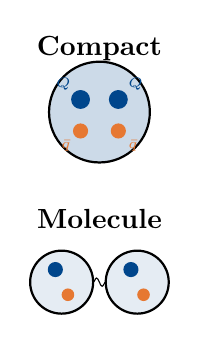
\begin{tikzpicture}[scale=0.8]
    % Compact tetraquark
    \node at (0,3.5) {\textbf{Compact}};
    \draw[thick,fill=heavyblue!20] (0,2.5) circle (0.8);
    \fill[heavyblue] (-0.3,2.7) circle (0.15) node[above left,font=\tiny] {$Q$};
    \fill[heavyblue] (0.3,2.7) circle (0.15) node[above right,font=\tiny] {$Q$};
    \fill[lightquarkorange] (-0.3,2.2) circle (0.12) node[below left,font=\tiny] {$\bar{q}$};
    \fill[lightquarkorange] (0.3,2.2) circle (0.12) node[below right,font=\tiny] {$\bar{q}$};

    % Molecule
    \node at (0,0.8) {\textbf{Molecule}};
    \draw[thick,fill=heavyblue!10] (-0.6,-0.2) circle (0.5);
    \draw[thick,fill=heavyblue!10] (0.6,-0.2) circle (0.5);
    \fill[heavyblue] (-0.7,0) circle (0.12);
    \fill[lightquarkorange] (-0.5,-0.4) circle (0.1);
    \fill[heavyblue] (0.5,0) circle (0.12);
    \fill[lightquarkorange] (0.7,-0.4) circle (0.1);
    \draw[decorate,decoration={snake,amplitude=1.5pt,segment length=4pt}] (-0.1,-0.2) -- (0.1,-0.2);
\end{tikzpicture}
\end{column}
\end{columns}
\end{frame}

%==============================================================================
% SLIDE 3: Computational Challenges
%==============================================================================
\begin{frame}{Computational Challenges in Multiquark Systems}
\begin{columns}[T]
\begin{column}{0.48\textwidth}
\textbf{Exponential Complexity:}
\begin{itemize}
    \item Wave function dimension scales exponentially with particle number
    \item Extra SU(3) color degree of freedom
    \item Multiple quantum numbers: $S$, $I$, $J^{PC}$, color
\end{itemize}

\vspace{0.5em}
\textbf{Strong Correlations:}
\begin{itemize}
    \item Single-particle approximation \textbf{fails}
    \item No shell structure (unlike atoms/nuclei)
    \item Full multi-channel dynamics required
\end{itemize}
\end{column}
\begin{column}{0.48\textwidth}
\textbf{Limitations of Existing Methods:}
\vspace{0.3em}

\textcolor{heavyblue}{\textbf{Gaussian Expansion Method (GEM):}}
\begin{itemize}
    \item Exponential growth of basis states
    \item Incomplete calculations for 5+ quarks
\end{itemize}

\vspace{0.3em}
\textcolor{heavyblue}{\textbf{Diffusion Monte Carlo (DMC):}}
\begin{itemize}
    \item Notorious \textbf{sign problem}
    \item Limited applicability to strongly correlated systems
\end{itemize}

\vspace{0.3em}
\textcolor{heavyblue}{\textbf{Previous Pentaquark Studies:}}
\begin{itemize}
    \item Approximations in spatial configurations
    \item Simplified color degree of freedom
    \item $\Rightarrow$ Unknown systematic errors
\end{itemize}
\end{column}
\end{columns}
\end{frame}

%==============================================================================
% SECTION 2: DEEP LEARNING BACKGROUND
%==============================================================================
\section{Deep Learning Background}

%==============================================================================
% SLIDE 4: What is Machine Learning?
%==============================================================================
\begin{frame}{What is Machine Learning?}
\begin{columns}[T]
\begin{column}{0.55\textwidth}
\textbf{Core Idea:}\\
Learn patterns from data without explicit programming

\vspace{0.5em}
\textbf{Types of Learning:}
\begin{itemize}
    \item \textbf{Supervised:} Learn from labeled examples\\
    {\small (classification, regression)}
    \item \textbf{Unsupervised:} Find hidden structure\\
    {\small (clustering, dimensionality reduction)}
    \item \textbf{Variational:} Optimize a target functional\\
    {\small $\Leftarrow$ \textbf{What we use!}}
\end{itemize}

\vspace{0.5em}
\textbf{Universal Approximation Theorem:}\\
Neural networks can approximate \textit{any} continuous function to arbitrary accuracy
\end{column}
\begin{column}{0.42\textwidth}
\centering
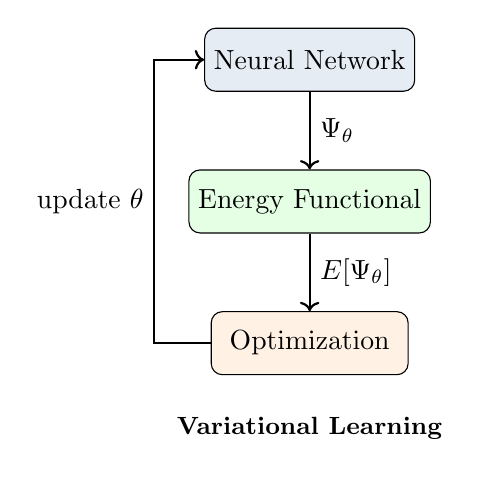
\begin{tikzpicture}[scale=0.9]
    % Variational optimization diagram
    \node[draw,rounded corners,fill=heavyblue!10,minimum width=2.5cm,minimum height=0.8cm] (model) at (0,2) {Neural Network};
    \node[draw,rounded corners,fill=green!10,minimum width=2.5cm,minimum height=0.8cm] (func) at (0,0) {Energy Functional};
    \node[draw,rounded corners,fill=orange!10,minimum width=2.5cm,minimum height=0.8cm] (opt) at (0,-2) {Optimization};

    \draw[->,thick] (model) -- node[right] {$\Psi_\theta$} (func);
    \draw[->,thick] (func) -- node[right] {$E[\Psi_\theta]$} (opt);
    \draw[->,thick] (opt.west) -- ++(-0.8,0) |- node[left,pos=0.25] {update $\theta$} (model.west);

    \node at (0,-3.2) {\small \textbf{Variational Learning}};
\end{tikzpicture}
\end{column}
\end{columns}
\end{frame}

%==============================================================================
% SLIDE 5: Neural Networks
%==============================================================================
\begin{frame}{Neural Networks: The Basic Building Block}
\begin{columns}[T]
\begin{column}{0.5\textwidth}
\textbf{Single Neuron:}
\begin{equation*}
y = \sigma(\mathbf{W}\mathbf{x} + \mathbf{c})
\end{equation*}
where $\sigma = \tanh$ (activation function)

\vspace{0.5em}
\centering
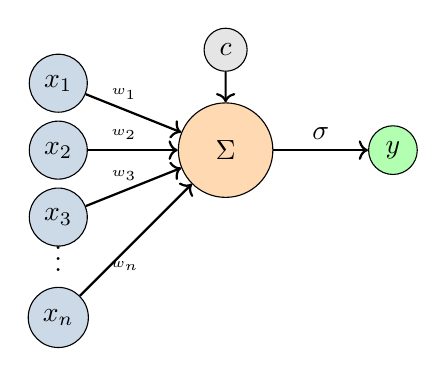
\begin{tikzpicture}[scale=0.85]
    % Input nodes
    \foreach \i in {1,2,3} {
        \node[circle,draw,fill=heavyblue!20,minimum size=0.6cm] (in\i) at (-2,2-\i) {$x_\i$};
    }
    \node at (-2,-1.5) {$\vdots$};
    \node[circle,draw,fill=heavyblue!20,minimum size=0.6cm] (in4) at (-2,-2.5) {$x_n$};

    % Neuron
    \node[circle,draw,fill=orange!30,minimum size=1.2cm] (neuron) at (0.5,0) {$\Sigma$};

    % Output
    \node[circle,draw,fill=green!30,minimum size=0.6cm] (out) at (3,0) {$y$};

    % Connections
    \foreach \i in {1,2,3} {
        \draw[->,thick] (in\i) -- node[above,font=\tiny,pos=0.4] {$w_\i$} (neuron);
    }
    \draw[->,thick] (in4) -- node[below,font=\tiny,pos=0.4] {$w_n$} (neuron);
    \draw[->,thick] (neuron) -- node[above] {$\sigma$} (out);

    % Bias
    \node[circle,draw,fill=gray!20,minimum size=0.4cm] (bias) at (0.5,1.5) {$c$};
    \draw[->,thick] (bias) -- (neuron);
\end{tikzpicture}
\end{column}
\begin{column}{0.48\textwidth}
\textbf{Physics Analogy: Basis Expansion}

\vspace{0.3em}
Traditional wave function:
\begin{equation*}
\Psi(x) = \sum_i c_i \phi_i(x)
\end{equation*}

Neural network:
\begin{equation*}
\Psi(x) = \sum_i w_i \sigma\left(\sum_j W_{ij} x_j + c_j\right)
\end{equation*}

\vspace{0.5em}
\textbf{Key difference:}
\begin{itemize}
    \item Basis functions $\phi_i$ are \textit{fixed} in traditional methods
    \item Neural network \textit{learns} the optimal basis!
    \item Adaptive, data-driven representation
\end{itemize}
\end{column}
\end{columns}
\end{frame}

%==============================================================================
% SLIDE 6: Deep Neural Networks
%==============================================================================
\begin{frame}{Deep Neural Networks: Stacking Layers}
\begin{columns}[T]
\begin{column}{0.55\textwidth}
\textbf{From Shallow to Deep:}
\begin{itemize}
    \item Multiple hidden layers between input and output
    \item Each layer transforms features progressively
    \item Deeper networks $\Rightarrow$ more complex functions
\end{itemize}

\vspace{0.5em}
\textbf{DeepQuark Architecture:}
\begin{itemize}
    \item \textbf{4 fully connected hidden layers}
    \item Layer sizes: $(32\text{--}40, 16\text{--}20, 16\text{--}20, 16\text{--}20)$
    \item \textbf{$\sim$1000--3000 parameters}
    \item Activation: $\sigma = \tanh$
\end{itemize}

\vspace{0.5em}
\textbf{Why ``Deep''?}
\begin{itemize}
    \item Efficiently captures hierarchical correlations
    \item Exponentially more expressive than shallow networks
\end{itemize}
\end{column}
\begin{column}{0.42\textwidth}
\centering
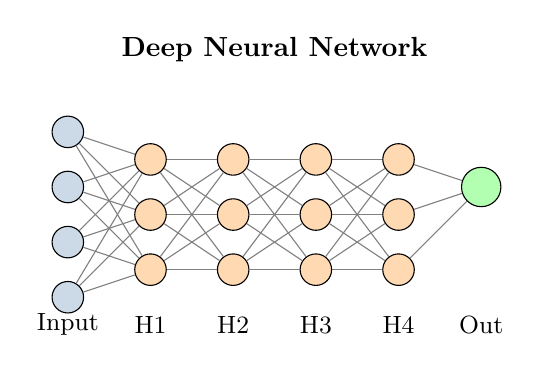
\begin{tikzpicture}[scale=0.7]
    % Input layer
    \foreach \i in {1,2,3,4} {
        \node[circle,draw,fill=heavyblue!20,minimum size=0.4cm] (in\i) at (0,3.5-\i) {};
    }
    \node at (0,-1) {\small Input};

    % Hidden layers
    \foreach \layer in {1,2,3,4} {
        \foreach \i in {1,2,3} {
            \node[circle,draw,fill=orange!30,minimum size=0.4cm] (h\layer\i) at (1.5*\layer,3-\i) {};
        }
    }
    \node at (1.5,-1) {\small H1};
    \node at (3,-1) {\small H2};
    \node at (4.5,-1) {\small H3};
    \node at (6,-1) {\small H4};

    % Output
    \node[circle,draw,fill=green!30,minimum size=0.5cm] (out) at (7.5,1.5) {};
    \node at (7.5,-1) {\small Out};

    % Connections (simplified)
    \foreach \i in {1,2,3,4} {
        \foreach \j in {1,2,3} {
            \draw[gray,thin] (in\i) -- (h1\j);
        }
    }
    \foreach \layer [evaluate=\layer as \nextlayer using int(\layer+1)] in {1,2,3} {
        \foreach \i in {1,2,3} {
            \foreach \j in {1,2,3} {
                \draw[gray,thin] (h\layer\i) -- (h\nextlayer\j);
            }
        }
    }
    \foreach \i in {1,2,3} {
        \draw[gray,thin] (h4\i) -- (out);
    }

    % Label
    \node at (3.75,4) {\textbf{Deep Neural Network}};
\end{tikzpicture}
\end{column}
\end{columns}
\end{frame}

%==============================================================================
% SLIDE 7: Neural Network Quantum States
%==============================================================================
\begin{frame}{Neural Network Quantum States (NNQS)}
\textbf{Key Insight:} Use neural networks to represent quantum wave functions
\begin{equation*}
\Psi(\mathbf{x}) = f_\text{NN}(\mathbf{x}; \boldsymbol{\theta})
\end{equation*}

\vspace{0.3em}
\begin{columns}[T]
\begin{column}{0.48\textwidth}
\textbf{Pioneering Work:}
\begin{itemize}
    \item \textbf{Carleo \& Troyer (2017):} Quantum spin systems with Restricted Boltzmann Machines
    \item \textbf{FermiNet (2020):} Ab initio molecular chemistry
    \item \textbf{PauliNet (2020):} Deep learning for quantum chemistry
\end{itemize}

\vspace{0.3em}
\textbf{Advantages:}
\begin{itemize}
    \item No fixed basis --- adaptive representation
    \item Captures complex many-body correlations
    \item Scalable to larger systems
\end{itemize}
\end{column}
\begin{column}{0.48\textwidth}
\textbf{Applications:}
\begin{itemize}
    \item Atomic \& molecular physics
    \item Condensed matter systems
    \item Nuclear physics (since 2020)
    \item \textcolor{heavyblue}{\textbf{Multiquark systems (this work!)}}
\end{itemize}

\vspace{0.3em}
\textbf{Why not applied to quarks before?}
\begin{itemize}
    \item Extra SU(3) color degree of freedom
    \item Strong correlations (no shell structure)
    \item Complex confinement interactions
\end{itemize}
\end{column}
\end{columns}
\end{frame}

%==============================================================================
% SLIDE 8: VMC Optimization
%==============================================================================
\begin{frame}{Variational Monte Carlo Optimization}
\begin{columns}[T]
\begin{column}{0.52\textwidth}
\textbf{Variational Principle:}
\begin{equation*}
E_{\boldsymbol{\theta}} = \frac{\langle\psi_{\boldsymbol{\theta}}|H|\psi_{\boldsymbol{\theta}}\rangle}{\langle\psi_{\boldsymbol{\theta}}|\psi_{\boldsymbol{\theta}}\rangle} \geq E_0
\end{equation*}
Minimize energy to find ground state!

\vspace{0.5em}
\textbf{Monte Carlo Evaluation:}
\begin{equation*}
E_{\boldsymbol{\theta}} \approx \frac{1}{N}\sum_{n=1}^N E_L(\mathbf{R}_n, \alpha_n)
\end{equation*}
Sample from $|\Psi(\mathbf{R},\alpha)|^2$

\vspace{0.5em}
\textbf{Stochastic Reconfiguration:}
\begin{equation*}
\boldsymbol{\theta}^{i+1} = \boldsymbol{\theta}^i - \eta(S+\epsilon I)^{-1}\nabla E
\end{equation*}
where $S$ is the quantum Fisher information matrix
\end{column}
\begin{column}{0.45\textwidth}
\centering
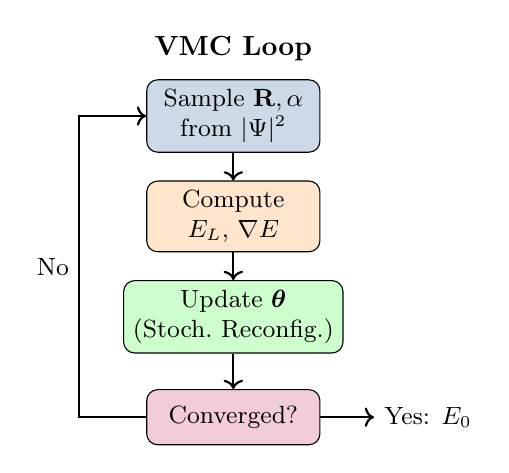
\begin{tikzpicture}[scale=0.85,
    box/.style={draw,rounded corners,minimum width=2.2cm,minimum height=0.7cm,align=center,font=\small}]

    \node[box,fill=heavyblue!20] (sample) at (0,3) {Sample $\mathbf{R},\alpha$\\from $|\Psi|^2$};
    \node[box,fill=orange!20] (compute) at (0,1.5) {Compute\\$E_L$, $\nabla E$};
    \node[box,fill=green!20] (update) at (0,0) {Update $\boldsymbol{\theta}$\\(Stoch.\ Reconfig.)};
    \node[box,fill=purple!20] (check) at (0,-1.5) {Converged?};

    \draw[->,thick] (sample) -- (compute);
    \draw[->,thick] (compute) -- (update);
    \draw[->,thick] (update) -- (check);
    \draw[->,thick] (check.west) -- ++(-1,0) |- node[left,pos=0.25] {\small No} (sample.west);
    \draw[->,thick] (check.east) -- ++(0.8,0) node[right] {\small Yes: $E_0$};

    \node at (0,4) {\textbf{VMC Loop}};
\end{tikzpicture}
\end{column}
\end{columns}

\vspace{0.3em}
\textbf{Key advantage:} No sign problem (unlike DMC)!
\end{frame}

%==============================================================================
% SECTION 3: DEEPQUARK FRAMEWORK
%==============================================================================
\section{DeepQuark Framework}

%==============================================================================
% SLIDE 9: DeepQuark Architecture
%==============================================================================
\begin{frame}{DeepQuark Architecture}
\centering
\includegraphics[width=0.85\textwidth]{arXiv-2506.20555v1/framework.pdf}

\vspace{0.3em}
\textbf{Four types of input:} Spatial coordinates $\mathbf{r}_i$, $|\mathbf{r}_i - \mathbf{r}_j|$ + Color $\alpha_c$ + Spin $\alpha_s$ + Isospin $\alpha_t$
\end{frame}

%==============================================================================
% SLIDE 10: Encoding Quantum Numbers
%==============================================================================
\begin{frame}{Encoding Quantum Numbers}
\begin{columns}[T]
\begin{column}{0.5\textwidth}
\textbf{Coupled Basis Representation:}\\
Color-spin-isospin bases for tetraquark $QQ\bar{q}\bar{q}$:
\begin{align*}
&\chi_{\bar{3}_c\otimes 3_c}\phi^{s_a,s_b}\xi^{I=0}=\left[(QQ)_{\bar{3}_c}^{s_a}(\bar{q}\bar{q})_{3_c}^{s_b,I=0}\right]_{1_c}^{S=1}\\[0.3em]
&\chi_{6_c\otimes \bar{6}_c}\phi^{s_a,s_b}\xi^{I=0}=\left[(QQ)_{6_c}^{s_a}(\bar{q}\bar{q})_{\bar{6}_c}^{s_b,I=0}\right]_{1_c}^{S=1}
\end{align*}

\vspace{0.3em}
\textbf{Why coupled bases?}
\begin{itemize}
    \item Automatically enforces symmetry
    \item Natural for strong correlations
    \item No single-particle approximation needed
\end{itemize}
\end{column}
\begin{column}{0.48\textwidth}
\textbf{One-Hot Encoding:}\\
Map discrete quantum numbers to vectors

\vspace{0.5em}
Example with 2 color bases:
\begin{align*}
\chi_{\bar{3}_c\otimes 3_c} &\rightarrow \alpha_c = (1, 0)\\
\chi_{6_c\otimes \bar{6}_c} &\rightarrow \alpha_c = (0, 1)
\end{align*}

\vspace{0.3em}
\textbf{Key insight:}\\
Standard basis vectors ensure no prejudiced correlation between different bases

\vspace{0.5em}
\textbf{Input features:}
\begin{equation*}
\mathbf{x} = (\mathbf{r}_i, |\mathbf{r}_i - \mathbf{r}_j|, \alpha_c, \alpha_s, \alpha_t)
\end{equation*}
\end{column}
\end{columns}
\end{frame}

%==============================================================================
% SLIDE 11: Symmetry Enforcement
%==============================================================================
\begin{frame}{Symmetry Enforcement}
\textbf{Full wave function with all symmetries:}
\begin{equation*}
\boxed{\Psi_{\text{A}}^\pi(\boldsymbol{x}) = (1+\pi\hat{P})\mathcal{A}\left[f_{NN}(\boldsymbol{x})\prod_{i<j}\exp\left(-\frac{r_{ij}^2}{b^2}\right)\right]}
\end{equation*}

\vspace{0.3em}
\begin{columns}[T]
\begin{column}{0.32\textwidth}
\textbf{Boundary Condition:}
\begin{equation*}
\prod_{i<j}e^{-r_{ij}^2/b^2}
\end{equation*}
\begin{itemize}
    \item Confines system to localized space
    \item $b = 2$--$4$ fm (order of $\Lambda_\text{QCD}^{-1}$)
    \item Ensures convergence from random initialization
\end{itemize}
\end{column}
\begin{column}{0.32\textwidth}
\textbf{Antisymmetrization:}
\begin{equation*}
\mathcal{A}[\cdots]
\end{equation*}
\begin{itemize}
    \item Enforces Fermi-Dirac statistics
    \item Sum over permutations of identical particles
    \item Factorial complexity, but manageable for 3--4 identical quarks
\end{itemize}
\end{column}
\begin{column}{0.32\textwidth}
\textbf{Parity Projection:}
\begin{equation*}
(1+\pi\hat{P})
\end{equation*}
\begin{itemize}
    \item Projects onto definite parity $\pi = \pm 1$
    \item $\hat{P}$: spatial inversion operator
    \item Ground states: positive parity (tetraquark), negative parity (pentaquark)
\end{itemize}
\end{column}
\end{columns}
\end{frame}

%==============================================================================
% SLIDE 12: Key Innovations
%==============================================================================
\begin{frame}{Key Innovations of DeepQuark}
\begin{columns}[T]
\begin{column}{0.48\textwidth}
\textbf{1. Coupled Bases vs.\ Determinant Ansatz}
\begin{itemize}
    \item Previous NNQS (FermiNet, PauliNet):\\ Slater determinants + Jastrow factors
    \item Originates from single-particle orbitals
    \item Works for weakly correlated systems
\end{itemize}

\vspace{0.3em}
\textbf{DeepQuark:}
\begin{itemize}
    \item Coupled color-spin-isospin bases
    \item No single-particle assumption
    \item Natural for strongly correlated hadrons
\end{itemize}
\end{column}
\begin{column}{0.48\textwidth}
\textbf{2. Unbiased Structure Description}
\begin{itemize}
    \item Same wave function ansatz describes:
    \begin{itemize}
        \item Compact tetraquarks ($T_{bb}$)
        \item Hadronic molecules ($T_{cc}$)
        \item Scattering states
    \end{itemize}
    \item No \textit{a priori} assumption about structure
    \item Network \textit{learns} the configuration!
\end{itemize}

\vspace{0.3em}
\textbf{3. Complex Interactions:}
\begin{itemize}
    \item Handles flux-tube confinement
    \item No extra computational cost
    \item Opens door to many-body forces
\end{itemize}
\end{column}
\end{columns}
\end{frame}

%==============================================================================
% SECTION 4: RESULTS
%==============================================================================
\section{Results}

%==============================================================================
% SLIDE 13: Nucleon Benchmarks
%==============================================================================
\begin{frame}{Benchmark: Nucleon with Different Confinements}
\begin{columns}[T]
\begin{column}{0.22\textwidth}
\centering
\includegraphics[width=\textwidth]{arXiv-2506.20555v1/qqqFT.pdf}

\vspace{0.2em}
{\scriptsize Confinement:\\
\textbf{L:} Pairwise\\
\textbf{R:} Flux-tube}
\end{column}
\begin{column}{0.76\textwidth}
\centering
\includegraphics[width=\textwidth]{arXiv-2506.20555v1/Graph_multiquark.pdf}

{\small (a) nucleon, (b) $T_{cc}$, (c) $T_{4c}$, (d) pentaquark --- DeepQuark matches GEM/DMC}
\end{column}
\end{columns}
\end{frame}

%==============================================================================
% SLIDE 14: Tcc Tetraquark
%==============================================================================
\begin{frame}{Doubly Charmed Tetraquark $T_{cc}$}
\begin{columns}[T]
\begin{column}{0.45\textwidth}
\centering
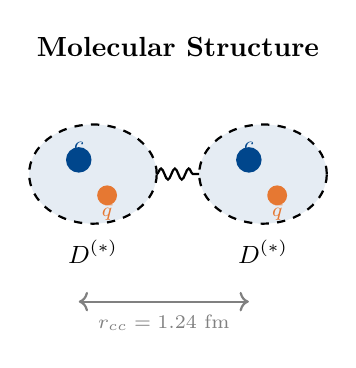
\begin{tikzpicture}[scale=0.9]
    % Molecular structure diagram
    \node at (0,3.8) {\textbf{Molecular Structure}};

    % Two mesons
    \draw[thick,dashed,fill=heavyblue!10] (-1.2,2) ellipse (0.9 and 0.7);
    \draw[thick,dashed,fill=heavyblue!10] (1.2,2) ellipse (0.9 and 0.7);

    % Quarks in left meson
    \fill[heavyblue] (-1.4,2.2) circle (0.18) node[above,font=\scriptsize] {$c$};
    \fill[lightquarkorange] (-1.0,1.7) circle (0.14) node[below,font=\scriptsize] {$\bar{q}$};

    % Quarks in right meson
    \fill[heavyblue] (1.0,2.2) circle (0.18) node[above,font=\scriptsize] {$c$};
    \fill[lightquarkorange] (1.4,1.7) circle (0.14) node[below,font=\scriptsize] {$\bar{q}$};

    % Interaction
    \draw[decorate,decoration={snake,amplitude=2pt,segment length=5pt},thick] (-0.3,2) -- (0.3,2);

    % Labels
    \node at (-1.2,0.9) {\small $D^{(*)}$};
    \node at (1.2,0.9) {\small $D^{(*)}$};

    % Distances
    \draw[<->,thick,gray] (-1.4,0.2) -- (1.0,0.2);
    \node[gray] at (-0.2,-0.1) {\scriptsize $r_{cc} = 1.24$ fm};
\end{tikzpicture}

\vspace{0.3em}
{\small See convergence plot: panel (b)}
\end{column}
\begin{column}{0.52\textwidth}
\textbf{Ground State Properties:}
\begin{itemize}
    \item Binding energy: $\Delta E = \mathbf{-15}$ MeV\\
    {\small (w.r.t.\ $D^*D$ threshold)}
    \item \textbf{Color mixing:} $\chi_{\bar{3}\times 3} : \chi_{6\times\bar{6}} = 55\% : 45\%$
    \item Significant mixing of both configurations!
\end{itemize}

\vspace{0.3em}
\textbf{RMS Radii (Molecular Structure):}
\begin{center}
\begin{tabular}{cc}
\toprule
$r_{c\bar{q}}$ & 1.06 fm\\
$r_{cc}$ & 1.24 fm\\
$r_{\bar{q}\bar{q}}$ & 1.41 fm\\
\bottomrule
\end{tabular}
\end{center}

$r_{cc}, r_{\bar{q}\bar{q}} > r_{c\bar{q}}$ $\Rightarrow$ \textbf{Molecular $D^*D$}

\vspace{0.3em}
Consistent with LHCb $T_{cc}(3875)^+$ discovery!
\end{column}
\end{columns}
\end{frame}

%==============================================================================
% SLIDE 15: Tbb Tetraquark
%==============================================================================
\begin{frame}{Doubly Bottom Tetraquark $T_{bb}$: Compact Diquark}
\begin{columns}[T]
\begin{column}{0.48\textwidth}
\textbf{Ground State Properties:}
\begin{itemize}
    \item Binding energy: $\Delta E = -153$ MeV\\
    {\small (w.r.t.\ $\bar{B}^*\bar{B}$ threshold)}
    \item \textbf{Color:} $\chi_{\bar{3}\times 3} : \chi_{6\times\bar{6}} = 97\% : 3\%$
    \item Dominated by $\bar{3}_c \otimes 3_c$ configuration!
\end{itemize}

\vspace{0.3em}
\textbf{Compact Structure:}
\begin{center}
\begin{tabular}{cc}
\toprule
$r_{bb}$ & \textbf{0.33 fm} (compact diquark!)\\
$r_{b\bar{q}}$ & 0.69 fm\\
$r_{\bar{q}\bar{q}}$ & 0.78 fm\\
\bottomrule
\end{tabular}
\end{center}

Heavy $bb$ diquark acts like $\bar{3}_c$ antiquark
\end{column}
\begin{column}{0.48\textwidth}
\centering
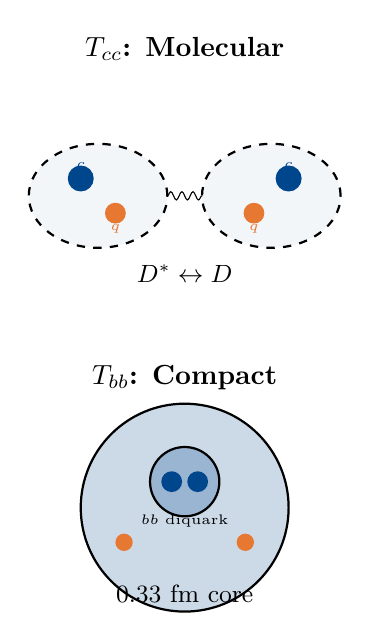
\begin{tikzpicture}[scale=1.1]
    % Tcc - molecular
    \node at (-1.5,3.5) {\textbf{$T_{cc}$: Molecular}};
    \draw[thick,dashed,fill=heavyblue!5] (-2.5,1.8) ellipse (0.8 and 0.6);
    \draw[thick,dashed,fill=heavyblue!5] (-0.5,1.8) ellipse (0.8 and 0.6);
    \fill[heavyblue] (-2.7,2) circle (0.15) node[above,font=\tiny] {$c$};
    \fill[lightquarkorange] (-2.3,1.6) circle (0.12) node[below,font=\tiny] {$\bar{q}$};
    \fill[heavyblue] (-0.3,2) circle (0.15) node[above,font=\tiny] {$c$};
    \fill[lightquarkorange] (-0.7,1.6) circle (0.12) node[below,font=\tiny] {$\bar{q}$};
    \draw[decorate,decoration={snake,amplitude=1.5pt,segment length=4pt}] (-1.7,1.8) -- (-1.3,1.8);
    \node at (-1.5,0.9) {\small $D^* \leftrightarrow D$};

    % Tbb - compact
    \node at (-1.5,-0.3) {\textbf{$T_{bb}$: Compact}};
    \draw[thick,fill=heavyblue!20] (-1.5,-1.8) circle (1.2);
    \draw[thick,fill=heavyblue!40] (-1.5,-1.5) circle (0.4);
    \fill[heavyblue] (-1.65,-1.5) circle (0.12);
    \fill[heavyblue] (-1.35,-1.5) circle (0.12);
    \node at (-1.5,-1.5) [below=0.3cm,font=\tiny] {$bb$ diquark};
    \fill[lightquarkorange] (-2.2,-2.2) circle (0.1);
    \fill[lightquarkorange] (-0.8,-2.2) circle (0.1);
    \node at (-1.5,-2.8) {\small 0.33 fm core};
\end{tikzpicture}
\end{column}
\end{columns}

\vspace{0.3em}
\textbf{Same ansatz} describes both molecular and compact structures!
\end{frame}

%==============================================================================
% SLIDE 16: Fully Heavy Tetraquarks
%==============================================================================
\begin{frame}{Fully Heavy Tetraquarks: $T_{4c}$ and $T_{4b}$}
\begin{columns}[T]
\begin{column}{0.45\textwidth}
\centering
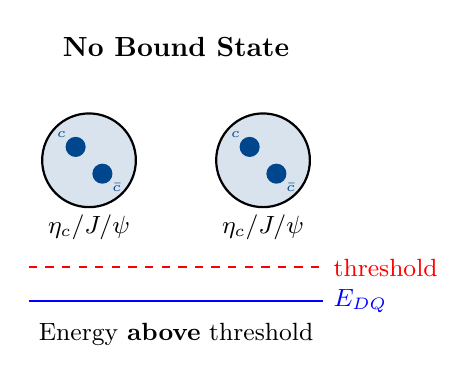
\begin{tikzpicture}[scale=0.85]
    % Scattering state diagram
    \node at (0,3.5) {\textbf{No Bound State}};

    % Two separate mesons
    \draw[thick,fill=heavyblue!15] (-1.3,1.8) circle (0.7);
    \draw[thick,fill=heavyblue!15] (1.3,1.8) circle (0.7);

    % Quarks
    \fill[heavyblue] (-1.5,2) circle (0.15) node[above left,font=\tiny] {$c$};
    \fill[heavyblue] (-1.1,1.6) circle (0.15) node[below right,font=\tiny] {$\bar{c}$};
    \fill[heavyblue] (1.1,2) circle (0.15) node[above left,font=\tiny] {$c$};
    \fill[heavyblue] (1.5,1.6) circle (0.15) node[below right,font=\tiny] {$\bar{c}$};

    % Labels
    \node at (-1.3,0.8) {\small $\eta_c/J/\psi$};
    \node at (1.3,0.8) {\small $\eta_c/J/\psi$};

    % Energy level
    \draw[dashed,thick,red] (-2.2,0.2) -- (2.2,0.2) node[right,font=\small] {threshold};
    \draw[thick,blue] (-2.2,-0.3) -- (2.2,-0.3) node[right,font=\small] {$E_{DQ}$};

    \node at (0,-0.8) {\small Energy \textbf{above} threshold};
\end{tikzpicture}

\vspace{0.2em}
{\small See convergence plot: panel (c)}
\end{column}
\begin{column}{0.52\textwidth}
\textbf{Results:}
\begin{center}
\begin{tabular}{lcc}
\toprule
System & $S^P$ & Bound?\\
\midrule
$cc\bar{c}\bar{c}$ & $0^+, 1^+, 2^+$ & \textbf{No}\\
$bb\bar{b}\bar{b}$ & $0^+, 1^+, 2^+$ & \textbf{No}\\
\bottomrule
\end{tabular}
\end{center}

\vspace{0.2em}
\textbf{Color proportion:} $\chi_{\bar{3}\times 3} : \chi_{6\times\bar{6}} \approx 1:2$\\
$\Rightarrow$ Consistent with meson-meson scattering

\vspace{0.4em}
\textbf{Experimental context:}
\begin{itemize}
    \item LHCb (2020): $T_{4c}(6900)$ resonance
    \item CMS (2025): Three $T_{4c}$ with $J^{PC} = 2^{++}$
\end{itemize}

\vspace{0.2em}
$\Rightarrow$ Observed structures are \textbf{resonances}, not bound states
\end{column}
\end{columns}
\end{frame}

%==============================================================================
% SLIDE 17: Pentaquark Overview
%==============================================================================
\begin{frame}{Triply Heavy Pentaquarks: $QQqq\bar{Q}$}
\begin{columns}[T]
\begin{column}{0.48\textwidth}
\textbf{Diquark-Antiquark Analogy:}

Heavy diquark $(QQ)_{\bar{3}_c}$ has same color as antiquark $\bar{Q}$

\vspace{0.3em}
\centering
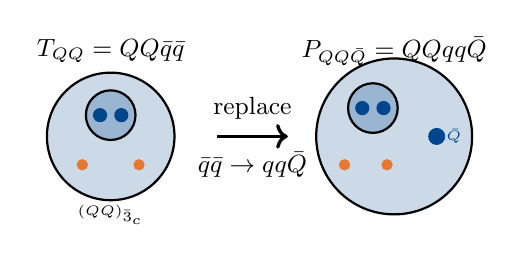
\begin{tikzpicture}[scale=0.9]
    % Tetraquark
    \node at (-1.5,2.5) {\small $T_{QQ} = QQ\bar{q}\bar{q}$};
    \draw[thick,fill=heavyblue!20] (-1.5,1.3) circle (0.9);
    \draw[thick,fill=heavyblue!40] (-1.5,1.6) circle (0.35);
    \fill[heavyblue] (-1.65,1.6) circle (0.1);
    \fill[heavyblue] (-1.35,1.6) circle (0.1);
    \fill[lightquarkorange] (-1.9,0.9) circle (0.08);
    \fill[lightquarkorange] (-1.1,0.9) circle (0.08);
    \node at (-1.5,0.2) {\tiny $(QQ)_{\bar{3}_c}$};

    % Arrow
    \draw[->,very thick] (0,1.3) -- (1,1.3);
    \node at (0.5,1.7) {\small replace};
    \node at (0.5,0.9) {\small $\bar{q}\bar{q} \to qq\bar{Q}$};

    % Pentaquark
    \node at (2.5,2.5) {\small $P_{QQ\bar{Q}} = QQqq\bar{Q}$};
    \draw[thick,fill=heavyblue!20] (2.5,1.3) circle (1.1);
    \draw[thick,fill=heavyblue!40] (2.2,1.7) circle (0.35);
    \fill[heavyblue] (2.05,1.7) circle (0.1);
    \fill[heavyblue] (2.35,1.7) circle (0.1);
    \fill[lightquarkorange] (1.8,0.9) circle (0.08);
    \fill[lightquarkorange] (2.4,0.9) circle (0.08);
    \fill[heavyblue] (3.1,1.3) circle (0.12) node[right,font=\tiny] {$\bar{Q}$};
\end{tikzpicture}
\end{column}
\begin{column}{0.48\textwidth}
\textbf{Color Bases for Pentaquark:}
\begin{align*}
\chi_{\bar{3}\otimes\bar{3}} &= \{[(QQ)_{\bar{3}}(qq)_{\bar{3}}]_{3}\bar{Q}\}_{1}\\
\chi_{\bar{3}\otimes 6} &= \{[(QQ)_{\bar{3}}(qq)_{6}]_{3}\bar{Q}\}_{1}\\
\chi_{6\otimes\bar{3}} &= \{[(QQ)_{6}(qq)_{\bar{3}}]_{3}\bar{Q}\}_{1}
\end{align*}

\vspace{0.3em}
\textbf{Expectation:}\\
If $T_{QQ}$ is bound, perhaps $P_{QQ\bar{Q}}$ is too?

\vspace{0.3em}
\textbf{Complication:}\\
$\bar{Q}$ can form quarkonium $(Q\bar{Q})_{1_c}$ with one of the heavy quarks --- lower energy configuration!
\end{column}
\end{columns}
\end{frame}

%==============================================================================
% SLIDE 18: Pentaquark S=1/2, 3/2
%==============================================================================
\begin{frame}{Pentaquarks with $S = 1/2, 3/2$: No Binding}
\begin{columns}[T]
\begin{column}{0.48\textwidth}
\textbf{Results for $S = 1/2, 3/2$:}
\begin{center}
\begin{tabular}{lcc}
\toprule
System & $S^P$ & Bound?\\
\midrule
$ccqq\bar{c}$ & $\frac{1}{2}^-, \frac{3}{2}^-$ & \textbf{No}\\
$bbqq\bar{b}$ & $\frac{1}{2}^-, \frac{3}{2}^-$ & \textbf{No}\\
\bottomrule
\end{tabular}
\end{center}

\vspace{0.3em}
\textbf{Lowest thresholds:}
\begin{itemize}
    \item $ccqq\bar{c}$: $\eta_c \Lambda_c$ or $J/\psi \Lambda_c$
    \item $bbqq\bar{b}$: $\eta_b \Lambda_b$ or $\Upsilon \Lambda_b$
\end{itemize}
\end{column}
\begin{column}{0.48\textwidth}
\textbf{Why no binding?}

The $\bar{Q}$ ``steals'' a heavy quark to form quarkonium:

\vspace{0.3em}
\centering
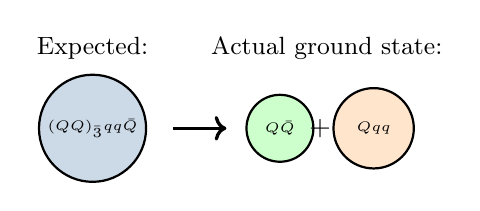
\begin{tikzpicture}[scale=0.85]
    % Initial
    \node at (0,2) {\small Expected:};
    \draw[thick,fill=heavyblue!20] (0,0.8) circle (0.8);
    \node at (0,0.8) {\tiny $(QQ)_{\bar{3}}qq\bar{Q}$};

    % Arrow
    \draw[->,very thick] (1.2,0.8) -- (2,0.8);

    % Final
    \node at (3.5,2) {\small Actual ground state:};
    \draw[thick,fill=green!20] (2.8,0.8) circle (0.5);
    \node at (2.8,0.8) {\tiny $Q\bar{Q}$};
    \node at (3.4,0.8) {$+$};
    \draw[thick,fill=orange!20] (4.2,0.8) circle (0.6);
    \node at (4.2,0.8) {\tiny $Qqq$};
\end{tikzpicture}

\vspace{0.5em}
$(Q\bar{Q})_{1_c}$ quarkonium + $(Qqq)$ baryon is more stable than $(QQ)_{\bar{3}_c}$ diquark configuration

\vspace{0.3em}
$\Rightarrow$ Diquark-antiquark symmetry is \textbf{broken}
\end{column}
\end{columns}
\end{frame}

%==============================================================================
% SLIDE 19: Novel Bound S=5/2 Pentaquarks
%==============================================================================
\begin{frame}{Novel Prediction: Bound $S = 5/2$ Pentaquarks}
\begin{columns}[T]
\begin{column}{0.45\textwidth}
\centering
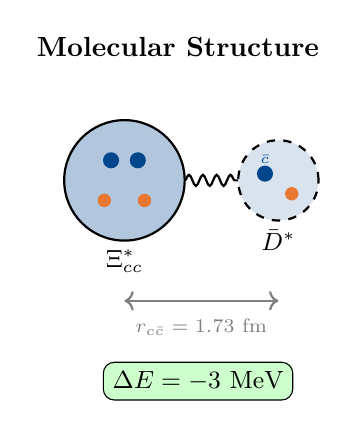
\begin{tikzpicture}[scale=0.85]
    % Title
    \node at (0,3.8) {\textbf{Molecular Structure}};

    % Xi_cc* baryon (compact)
    \draw[thick,fill=heavyblue!30] (-0.8,1.8) circle (0.9);
    \fill[heavyblue] (-1.0,2.1) circle (0.12);
    \fill[heavyblue] (-0.6,2.1) circle (0.12);
    \fill[lightquarkorange] (-1.1,1.5) circle (0.1);
    \fill[lightquarkorange] (-0.5,1.5) circle (0.1);
    \node at (-0.8,0.6) {\small $\Xi_{cc}^*$};

    % D* meson
    \draw[thick,dashed,fill=heavyblue!15] (1.5,1.8) circle (0.6);
    \fill[heavyblue] (1.3,1.9) circle (0.12) node[above,font=\tiny] {$\bar{c}$};
    \fill[lightquarkorange] (1.7,1.6) circle (0.1);
    \node at (1.5,0.9) {\small $\bar{D}^*$};

    % Interaction
    \draw[decorate,decoration={snake,amplitude=2pt,segment length=5pt},thick] (0.1,1.8) -- (0.9,1.8);

    % Distance annotation
    \draw[<->,thick,gray] (-0.8,0.0) -- (1.5,0.0);
    \node[gray] at (0.35,-0.4) {\scriptsize $r_{c\bar{c}} = 1.73$ fm};

    % Binding
    \node[draw,rounded corners,fill=green!20] at (0.3,-1.2) {\small $\Delta E = -3$ MeV};
\end{tikzpicture}

{\small See convergence plot: panel (d)}
\end{column}
\begin{column}{0.52\textwidth}
\textbf{Why $S = 5/2$ is special:}\\
S-wave $S=\frac{3}{2}$ isoscalar baryon is \textbf{forbidden} by Fermi statistics!

\vspace{0.2em}
$\Rightarrow$ Lowest threshold: $\bar{D}^*\Xi_{cc}^*$ (or $B^*\Xi_{bb}^*$)

\vspace{0.4em}
\textbf{Bound states found:}
\begin{center}
\begin{tabular}{lcc}
\toprule
State & Mass & $\Delta E$\\
\midrule
$P_{cc\bar{c}}(5715)$ & 5715 MeV & $\mathbf{-3}$ MeV\\
$P_{bb\bar{b}}(15569)$ & 15569 MeV & $\mathbf{-14}$ MeV\\
\bottomrule
\end{tabular}
\end{center}

\vspace{0.2em}
\textbf{Structure:} Molecular $\bar{D}^*\Xi_{cc}^*$
\begin{itemize}
    \item $r_{cc} = 0.50$ fm (compact $\Xi_{cc}^*$)
    \item $r_{c\bar{c}} = 1.73$ fm (large separation)
\end{itemize}

$\Rightarrow$ Analogous to molecular $T_{cc}$!
\end{column}
\end{columns}
\end{frame}

%==============================================================================
% SLIDE 20: Experimental Search
%==============================================================================
\begin{frame}{Experimental Search for $P_{cc\bar{c}}(5715)$}
\begin{columns}[T]
\begin{column}{0.55\textwidth}
\textbf{Decay Channels:}

$P_{cc\bar{c}}(5715)$ with $J^P = \frac{5}{2}^-$ can decay to lower-spin channels via spin-orbit coupling:

\vspace{0.3em}
\begin{itemize}
    \item Primary search channel: $\boxed{J/\psi\, \Lambda_c}$
    \item Requires \textbf{D-wave} decay (angular momentum barrier)
\end{itemize}

\vspace{0.5em}
\textbf{Expected Properties:}
\begin{itemize}
    \item \textbf{Narrow width} due to D-wave suppression
    \item Mass: $\sim 5715$ MeV
    \item Quantum numbers: $J^P = \frac{5}{2}^-$, $I = 0$
\end{itemize}

\vspace{0.5em}
\textbf{Production:}\\
Similar to $P_c$ pentaquarks at LHCb\\
$\Lambda_b \to J/\psi\, \Lambda_c\, K^-$ (or similar)
\end{column}
\begin{column}{0.42\textwidth}
\textbf{Properties of $P_{cc\bar{c}}(5715)$:}
\begin{center}
\begin{tabular}{lc}
\toprule
Property & Value\\
\midrule
Mass & 5715 MeV\\
$\Delta E$ & $-3$ MeV\\
$J^P$ & $\frac{5}{2}^-$\\
Isospin & 0\\
\midrule
$r_{QQ}$ & 0.50 fm\\
$r_{Qq}$ & 1.39 fm\\
$r_{qq}$ & 1.90 fm\\
$r_{Q\bar{Q}}$ & 1.73 fm\\
$r_{q\bar{Q}}$ & 1.38 fm\\
\bottomrule
\end{tabular}
\end{center}

\vspace{0.3em}
Molecular $\bar{D}^*\Xi_{cc}^*$ structure
\end{column}
\end{columns}
\end{frame}

%==============================================================================
% SECTION 5: CONCLUSIONS
%==============================================================================
\section{Conclusions}

%==============================================================================
% SLIDE 21: Summary
%==============================================================================
\begin{frame}{Summary}
\textbf{DeepQuark:} First DNN-based VMC for multiquark bound states

\vspace{0.5em}
\begin{columns}[T]
\begin{column}{0.48\textwidth}
\textbf{Method Achievements:}
\begin{itemize}
    \item Novel architecture with coupled color-spin-isospin bases
    \item Unbiased description of compact \& molecular states
    \item Handles flux-tube confinement efficiently
    \item Competitive with GEM and DMC
    \item Scalable to larger systems
\end{itemize}
\end{column}
\begin{column}{0.48\textwidth}
\textbf{Physics Results:}
\begin{itemize}
    \item \textbf{$T_{cc}$}: Molecular, $\Delta E = -15$ MeV, 55:45 color mixing
    \item \textbf{$T_{bb}$}: Compact diquark, $\Delta E = -153$ MeV, 97\% $\bar{3}\times 3$
    \item \textbf{$T_{4c}, T_{4b}$}: No bound states
    \item \textbf{New predictions:}
    \begin{itemize}
        \item $P_{cc\bar{c}}(5715)$: $-3$ MeV
        \item $P_{bb\bar{b}}(15569)$: $-14$ MeV
    \end{itemize}
    \item Search in D-wave $J/\psi\,\Lambda_c$
\end{itemize}
\end{column}
\end{columns}
\end{frame}

%==============================================================================
% SLIDE 22: Outlook
%==============================================================================
\begin{frame}{Outlook and Future Directions}
\begin{columns}[T]
\begin{column}{0.48\textwidth}
\textbf{Immediate Extensions:}
\begin{itemize}
    \item Other pentaquark systems ($P_c$, $P_b$)
    \item \textbf{Hexaquarks} (6 quarks)
    \item Excited states and resonances
    \item Different quark model potentials
\end{itemize}

\vspace{0.5em}
\textbf{Confinement Physics:}
\begin{itemize}
    \item Flux-tube interactions in tetraquarks
    \item Many-body confinement mechanisms
    \item Connection to lattice QCD results
\end{itemize}
\end{column}
\begin{column}{0.48\textwidth}
\textbf{Methodological Improvements:}
\begin{itemize}
    \item More sophisticated network architectures
    \item Excited state methods (penalty, orthogonalization)
    \item Scattering state descriptions
\end{itemize}

\vspace{0.5em}
\textbf{Broader Impact:}
\begin{itemize}
    \item Forward-looking predictions for experiments
    \item Insights into nonperturbative QCD
    \item General quantum many-body physics
    \item Deep learning + physics integration
\end{itemize}
\end{column}
\end{columns}
\end{frame}

%==============================================================================
% SLIDE 23: Acknowledgments
%==============================================================================
\begin{frame}{Acknowledgments}
\begin{columns}[T]
\begin{column}{0.55\textwidth}
\textbf{Collaborators:}
\begin{itemize}
    \item Wei-Lin Wu (Peking University)
    \item Shi-Lin Zhu (Peking University)
\end{itemize}

\vspace{0.5em}
\textbf{Helpful Discussions:}
\begin{itemize}
    \item Yao Ma, Yan-Ke Chen, Liang-Zhen Wen
    \item Yilong Yang, Pengwei Zhao
\end{itemize}

\vspace{0.5em}
\textbf{Funding:}
\begin{itemize}
    \item NSFC (No.\ 12475137)
    \item ERC NuclearTheory (Grant No.\ 885150)
\end{itemize}

\vspace{0.5em}
\textbf{Computing:}\\
High-performance Computing Platform of Peking University

\textbf{Software:} NetKet package
\end{column}
\begin{column}{0.4\textwidth}
\centering
\vspace{1cm}
\textbf{\Large Thank you!}

\vspace{1cm}
\textbf{Paper:}\\
arXiv:2506.20555

\vspace{0.5cm}
\textbf{Contact:}\\
lu.meng@rub.de
\end{column}
\end{columns}
\end{frame}

%==============================================================================
% BACKUP SLIDES
%==============================================================================
\appendix
\section{Backup}

%==============================================================================
% BACKUP B1: AL1 Model Parameters
%==============================================================================
\begin{frame}{Backup: AL1 Model Parameters}
\textbf{AL1 Quark Potential Model} (Semay \& Silvestre-Brac, 1996):
\begin{equation*}
V_{ij} = V_\text{OGE} + V_\text{conf} = -\frac{3}{16}\boldsymbol{\lambda}_i\cdot\boldsymbol{\lambda}_j\left(-\frac{\kappa}{r_{ij}} - \Lambda + \frac{8\pi\kappa'}{3m_im_j}\frac{e^{-r_{ij}^2/r_0^2}}{\pi^{3/2}r_0^3}\mathbf{s}_i\cdot\mathbf{s}_j + \lambda r_{ij}\right)
\end{equation*}

\vspace{0.3em}
\begin{center}
\begin{tabular}{cccccc}
\toprule
$\kappa$ & $\lambda$ (GeV$^2$) & $\Lambda$ (GeV) & $\kappa'$ & $m_b$ (GeV) & $m_c$ (GeV)\\
\midrule
0.5069 & 0.1653 & 0.8321 & 1.8609 & 5.227 & 1.836\\
\bottomrule
\end{tabular}
\end{center}

\begin{center}
\begin{tabular}{ccccc}
\toprule
$m_q$ (GeV) & $r_0$ (GeV$^{-1}$) & $A$ (GeV$^{B-1}$) & $B$ & $C$ (GeV$^4$)\\
\midrule
0.315 & $A(2m_im_j/(m_i+m_j))^{-B}$ & 1.6553 & 0.2204 & $2.02\times 10^{-3}$\\
\bottomrule
\end{tabular}
\end{center}
\end{frame}

%==============================================================================
% BACKUP B2: Detailed Color Bases
%==============================================================================
\begin{frame}{Backup: SU(3) Color Bases}
\textbf{Tetraquark $QQ\bar{q}\bar{q}$:}
\begin{align*}
(QQ): \quad &3 \otimes 3 = \bar{3} \oplus 6\\
(\bar{q}\bar{q}): \quad &\bar{3} \otimes \bar{3} = 3 \oplus \bar{6}\\
\text{Color singlet}: \quad &\bar{3} \otimes 3 = 1 \quad \text{and} \quad 6 \otimes \bar{6} \supset 1
\end{align*}

\textbf{Pentaquark $QQqq\bar{Q}$:}
\begin{align*}
\chi_{\bar{3}\otimes\bar{3}} &= \{[(QQ)_{\bar{3}}(qq)_{\bar{3}}]_{3}\bar{Q}\}_{1}\\
\chi_{\bar{3}\otimes 6} &= \{[(QQ)_{\bar{3}}(qq)_{6}]_{3}\bar{Q}\}_{1}\\
\chi_{6\otimes\bar{3}} &= \{[(QQ)_{6}(qq)_{\bar{3}}]_{3}\bar{Q}\}_{1}
\end{align*}

\textbf{Note:} $\chi_{6\otimes 6}$ does not contribute to color singlet
\end{frame}

%==============================================================================
% BACKUP B3: Optimization Details
%==============================================================================
\begin{frame}{Backup: Optimization Details}
\textbf{Network Architecture:}
\begin{center}
\begin{tabular}{lccc}
\toprule
System & $S^P$ & Nodes & Parameters\\
\midrule
$qqq$ & $\frac{1}{2}^+$ & $(16,16,16,16)$ & 1105\\
$QQ\bar{q}\bar{q}$ & $1^+$ & $(32,16,16,16)$ & 1889\\
$QQ\bar{Q}\bar{Q}$ & $0^+,1^+,2^+$ & $(32,16,16,16)$ & 1793--1857\\
$QQqq\bar{Q}$ & $\frac{1}{2}^-,\frac{3}{2}^-,\frac{5}{2}^-$ & $(40,20,20,20)$ & 2921--3081\\
\bottomrule
\end{tabular}
\end{center}

\textbf{Training:}
\begin{itemize}
    \item Initial: $N = 2\times 10^4$ samples (fast exploration)
    \item Convergence: $N = 4\text{--}8\times 10^4$ samples (stable optimization)
    \item Final evaluation: $N \sim 10^6$ samples
    \item Learning rate $\eta$, regularization $\epsilon = 10^{-3}$
    \item Stochastic reconfiguration with quantum Fisher matrix
\end{itemize}
\end{frame}

%==============================================================================
% BACKUP B4: Electron Benchmarks
%==============================================================================
\begin{frame}{Backup: Electron System Benchmarks}
\textbf{Few-electron systems as QED counterparts:}

\begin{center}
\begin{tabular}{lccc}
\toprule
System & DeepQuark (eV) & Reference (eV) & Difference\\
\midrule
$e^+e^-$ (Ps) & $-6.80301(16)$ & $-6.803$ (exact) & $<0.01\%$\\
$e^+e^-e^-$ (Ps$^-$) & $-7.12882(16)$ & $-7.130$ & $0.02\%$\\
$e^+e^+e^-e^-$ (Ps$_2$) & $-14.0347(7)$ & $-14.04$ & $0.04\%$\\
\bottomrule
\end{tabular}
\end{center}

\vspace{0.5em}
\textbf{Comparison methods:}
\begin{itemize}
    \item Ps: Exact solution (hydrogen-like)
    \item Ps$^-$: Hylleraas-type variational (Ho, 1993)
    \item Ps$_2$: Explicitly correlated Gaussians (Kinghorn \& Poshusta, 1993)
\end{itemize}

$\Rightarrow$ DeepQuark achieves $<0.1\%$ accuracy on all benchmarks
\end{frame}

%==============================================================================
% BACKUP B5: Comparison with FermiNet/PauliNet
%==============================================================================
\begin{frame}{Backup: DeepQuark vs.\ FermiNet/PauliNet}
\begin{center}
\begin{tabular}{lcc}
\toprule
Feature & FermiNet/PauliNet & DeepQuark\\
\midrule
Target systems & Atoms, molecules & Multiquark hadrons\\
Wave function & Slater determinants & Coupled bases\\
& + Jastrow + backflow & \\
Basis assumption & Single-particle orbitals & None (fully correlated)\\
Color DOF & N/A & Full SU(3) treatment\\
Typical parameters & $\sim 10^5$--$10^6$ & $\sim 10^3$\\
Correlations & Via backflow transform & Encoded in bases\\
Antisymmetry & Determinant structure & Explicit permutations\\
\bottomrule
\end{tabular}
\end{center}

\vspace{0.5em}
\textbf{Key difference:}
\begin{itemize}
    \item FermiNet/PauliNet: Determinant ansatz from atomic/molecular physics
    \item DeepQuark: Coupled basis construction for strongly correlated hadrons
\end{itemize}
\end{frame}

\end{document}
